\documentclass[a4paper,12pt,oneside,titlepage]{article} 
\usepackage[T1]{fontenc}
\usepackage[english]{babel}
\usepackage[utf8]{inputenc}
\usepackage{amsfonts} 
\usepackage{amssymb}
\usepackage{amsthm}
\usepackage{amsmath}
\usepackage{graphicx}
\usepackage{array}
\usepackage{booktabs}
\usepackage{siunitx}
\sisetup{output-decimal-marker={.}}
\usepackage{bm}
\usepackage{mathrsfs}
\usepackage[numbers]{natbib}
\usepackage{epstopdf}
\usepackage{subfig}
%\usepackage{subfloat}
\usepackage{multirow}
\usepackage{bm}
\usepackage{float}

\usepackage{verbatim}
\usepackage{hyperref}
\hypersetup{
	colorlinks=true,
	linkcolor=black,
	filecolor=magenta,      
	urlcolor=black,
}
\usepackage{caption}
\graphicspath{{images/}}            %path image
\captionsetup{tableposition=top,figureposition=bottom,format=hang, font=scriptsize}
\usepackage[skip=2pt]{caption}
\usepackage{cleveref}

%\captionsetup{format=myformat}

%\documentclass[paper=a4]{scrartcl}
\usepackage[utf8]{inputenc}
\usepackage[T1]{fontenc}
\usepackage[section]{placeins}
%\usepackage[showframe]{geometry}
%\usepackage{layout}
\setlength{\voffset}{0in}
%\setlength{\headsep}{5pt}
%\textwidth{600}
%\usepackage[a4paper]{geometry}
\usepackage{calc}
\usepackage[textheight=50\baselineskip+10pt]{geometry}

\begin{document}
	
	\thispagestyle{empty}
	\setcounter{page}{0}
	
	\begin{center}
		\huge
		POLITECNICO DI TORINO\\[1.cm]
		\Large
		ICT for Health \\
		\vspace{0.5cm}
		\Large
		Report Laboratory 2\\[1.3cm]
		
		\vspace{0.5cm}
		
\includegraphics[scale=2]{logo.jpg}
	\end{center}
	\vspace{1.cm}
	
	\begin{flushleft}
		\Large
		\noindent {\bfseries Professor:}\\
		Monica Visintin\\[0.2cm]
	\end{flushleft}
	\vspace{1cm}
	
	
	\begin{flushright} 
		\Large
		\noindent{\textbf{Student}:}\\
		Iman Ebrahimi Mehr S250190\\[0.2cm]
	\end{flushright} 
	\vspace{2cm}
	\begin{center}
		\Large
		A.Y.2019-2020
	\end{center}
	
	\newpage
	\thispagestyle{empty}
	\tableofcontents
	
	
	\newpage
	\section{Introduction}
	
	\textbf{Melanoma} is the most dangerous type of skin cancer that develops from the pigment-containing cells known as melanocytes. Melanomas typically occur in the skin, but may rarely occur in the mouth, intestines or eye. Sometimes they develop from a mole with changes such as an increase in size, irregular edges, change in color, itchiness or skin breakdown.
	
	ICT can be extremely useful in mole diagnosis. Having a software able to detect abnormalities saves time for the doctor and the patients. In fact, patients would not need to go to the hospitals for analysis, because they could send to the doctor a simple photo of the mole, and doctors can rely on machines doing basics analysis. It is important to say however, that machines cannot replace the doctor, that is fundamental in supervising the software results. 
	
	In the diagnosis of melanoma, five features are considered: A asymmetry; B border; C color; D diameter; E evolution. Forming the abbreviation ABCDE , easy to remember.
	
	
	\section{ICT in mole diagnosis}
	The scope of this lab is to analyze borders of a set of moles and melanomas starting from the its photography. The work outline includes the following steps idea is to: highlight the darkest part of the image, corresponding to the mole; find the contour of this darkest part; evaluate the length of the found contour (perimeter of the mole) and evaluate the ratio between the perimeter of the mole and the perimeter of the corresponding circle with the same area. In fact, this last calculation gives us an approximative information about the analyze mole: the lower the ratio (more regular mole's shape) if the ratio is very low, this means that the mole shouldn’t be a melanoma, otherwise it should be.
	
	
	\subsection{The data set}
	The software implemented in this place focuses on moles' border calculation. In particular, the irregularity of the mole border can be sign of abnormalities of that mole. The more the border is irregular, the higher the risk of melanoma. 
	
	The dataset is composed by 58 images of moles with different melanoma gravity risk level: low level, medium level and melanoma. For each of those, the border of the mole is isolated and compared to the perimeter of a circle with the same area, to check irregularity. 
	\subsection{Algorithm}
	\subsubsection{Preprocessing}
	First of all each photo is converted into quantized images(figure \ref{quantizied}) by using K-means in scikit-learn tool in python. The level of quantization depends on the image itself. Once done, the image is converted in binary representation: 1 indicates the mole (yellow pixels) and 0 represents the skin (violet pixels) (figure \ref{binary}).
	\begin{figure}[H]
		\centering
		\subfloat[][]{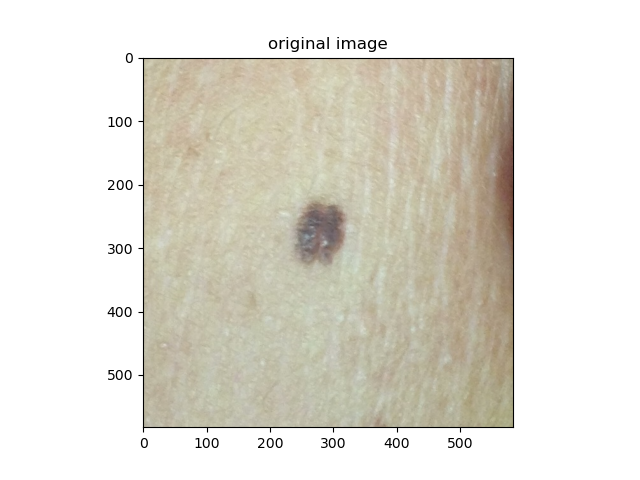
\includegraphics[scale=.3]{low_risk_4_original_image.png}\label{original}}
		\hfill
		\subfloat[][]{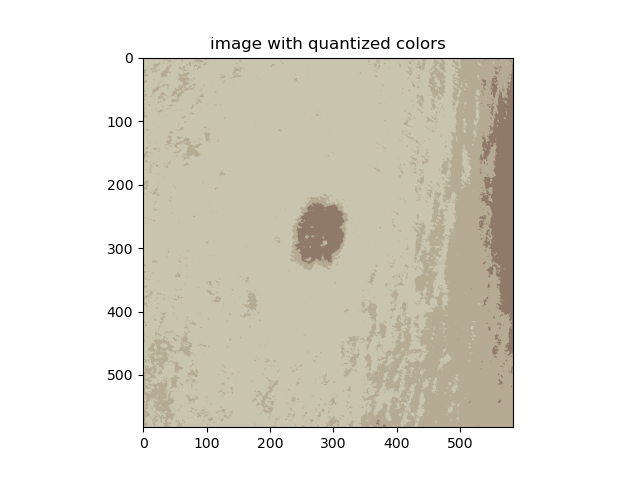
\includegraphics[scale=.3]{low_risk_4_image_with_quantized_colors.png}\label{quantizied}}
		\hfill
		\subfloat[][]{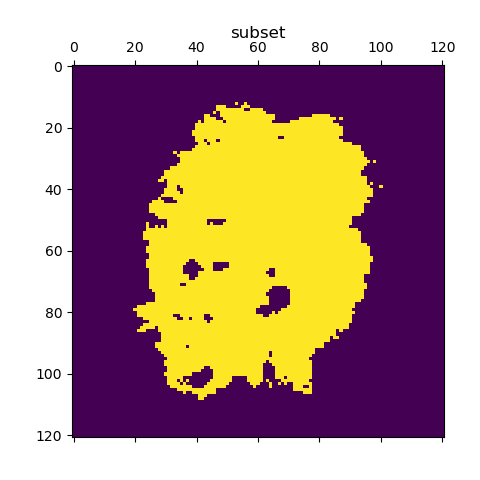
\includegraphics[scale=.3]{low_risk_4_subset.png}\label{binary}}
		\caption{moles}
		\label{pre_processing}
	\end{figure}
	
	
	The problem is that the image is not always 'clean': the mole sometimes contains violet pixels (caused by reflected light) and the skin sometimes contains yellow pixels (cause by some darker zones). Hence, data cleaning is required. \\
	The data cleaning process is made by analyzing pixel by pixel. It is divided in three parts: \textbf{noise removal}, \textbf{island correction} and \textbf{hole filling}. The \textbf{noise} consists in a number of scattered pixels that are not useful to outline the shape of the mole; the \textbf{the islands} are errors related to dark skin detected as mole; the \textbf{the holes} are errors related to light reflected on the mole (image \ref{example} reports the three kind of errors).
	
	\begin{figure}[ht]
		\centering
		\subfloat[][]{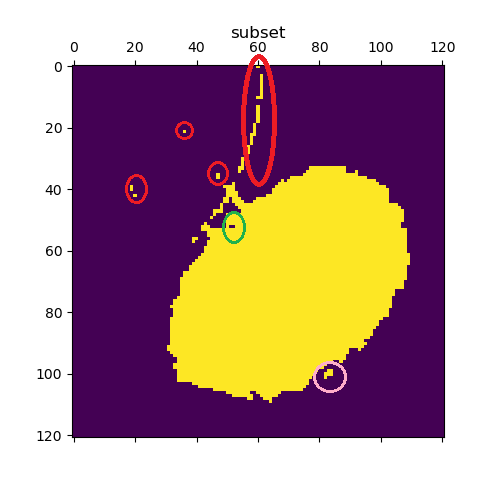
\includegraphics[scale=.34]{low_risk_3_s_subset_cc.png}\label{example}}
		\hspace{2cm}
		\subfloat[][]{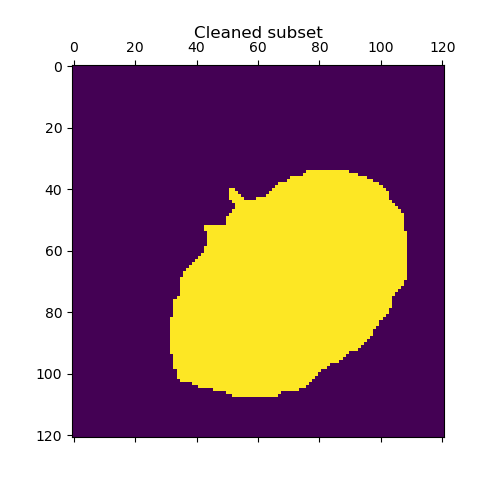
\includegraphics[scale=.34]{low_risk_3_s_Cleaned_subset.png}\label{cleaned}}
		
		\caption{\ref{example}Example of dirty image. The red circle highlights scattered pixels (noise); the green circle highlights hole error and pink circle highlights island error. The figure refers to the image: $'low_risk_3'$. Example of cleaned image (\ref{cleaned}). The image refers to the image \ref{cleaned} }
		
		
	\end{figure}
	
	\textbf{Part I: noise removal}.\\
	For each pixel the nearest neighbors are considered: 
	\begin{itemize}
		\item for the 4 corners' pixels: if the pixel in question has value 1 and at least two of its tree neighbors are 0 also the pixel in question should be 0, so it is modified from 1 to 0 (and vice versa). 
		\item for the frame pixels: if the pixel in question has value 1 and at least four of its five neighbors are 0 also the pixel in question should be 0, so it is modified from 1 to 0 (and vice versa). 
		\item for the internal pixels: if the pixel in question has value 1 and at least six of its eight neighbors are 0 also the pixel in question should be 0, so it is modified from 1 to 0 (and vice versa).  
	\end{itemize}
	
	\textbf{Part II and III : island correction and hole filling}.\\
	This part is carried out exactly like the first one, but the threshold in the number of neighbors to consider is lower. This makes sense because the scattered yellow pixels  are completely surrounded  by violet pixels, hence the number of neighbor with opposite value is higher. 
	
	In the end, the cleaned image shows up as reported in the image \ref{cleaned}
	
	
	
	\subsubsection{Perimeter calculation}
	Having at this point the cleaned image, it was possible to proceed with the perimeter calculation. The used approach is a basic one: for each pixel, again the neighbors are considered; if the pixel in yellow (value 1) and all the 4 neighbors are also yellow, it is considered as an internal pixel (internal to the mole), and, in another matrix, at the same position of the pixel in question, value 0 is assigned. Instead, if the yellow pixel has at least one violet neighbor this means that that pixel is a perimeter pixel and nothing happens.
	In the end, the image that is obtained shows up as in figure \ref{perimeter} where the inner part of the mole is completely removed and only the perimeter stands.
	
	\begin{figure}[H]
		\centering
		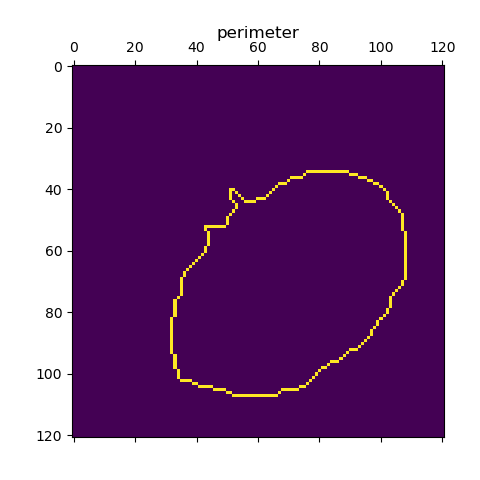
\includegraphics[scale=0.55]{low_risk_3_s_perimeter.png}
		
		\caption{Final image highlighting the perimeter.}
		\label{perimeter}
	\end{figure}
	
	
	\subsection{Results}
	All the moles' photos have been processed in this way. In the end, the perimeter of the mole is compared with the perimeter of the circle with the same area, as already mentioned in previous section. All the ratio are reported in the table below (\ref{table1}).
	
	
	\begin{table}[H]\footnotesize
		\begin{minipage}[b]{0.5\linewidth}%\centering
			\begin{tabular}{|c|c|c|c|}
				\hline
				\textbf{Image}  & \textbf{Mole} & \textbf{Circle} & \textbf{Ratio} \\
				\hline
				low\_risk\_1                          &326                     &326.68         &0.997\\
				low\_risk\_2                          &327                     &360.34         &0.935\\
				low\_risk\_3                          &281                     &254.19         &1.105\\
				low\_risk\_4                          &273                     &261.53         &1.043\\
				low\_risk\_5                          &252                     &246.87         &1.020\\
				low\_risk\_6                          &278                     &287.74        &0.966\\
				low\_risk\_7                          &215                     &195.09         &1.102\\
				low\_risk\_8                          &324                     &301.27       &1.075\\
				low\_risk\_9                          &184                     &203.29         &0.905\\
				low\_risk\_10                         &129                     &138.65         &0.930\\
				low\_risk\_11                         &192                     &202.83          &0.946\\
				medium\_risk\_1                       &117            &128.84      &0.908\\
				medium\_risk\_2                       &323            &333.57      &0.968\\
				medium\_risk\_3                       &160            &169.30      &0.945\\
				medium\_risk\_4                       &183            &185.18      &0.988\\
				medium\_risk\_5                       &651            &513.98      &1.266\\
				medium\_risk\_6                       &357            &315.11      &1.132\\
				medium\_risk\_7                       &671            &636.05      &1.054\\
				medium\_risk\_8                       &429                    &419.49      &1.022\\
				medium\_risk\_9                       &295            &235.72      &1.251\\
				medium\_risk\_10                      &421                    &388.51      &1.083\\
				medium\_risk\_11                       &608                    &591.37      &1.028\\
				medium\_risk\_12                      &405                    &432.27      &0.936\\
				medium\_risk\_13                      &293                    &291.26      &1.005\\
				medium\_risk\_14                      &336                    &349.65      &0.960\\
				medium\_risk\_15                      &325                    &320.75      &1.013\\
				medium\_risk\_16                      &471                    &483.03      &0.975\\
				\hline
			\end{tabular}
		\end{minipage}
		\hspace{0.6cm}
		\begin{minipage}[b]{0.1\linewidth}
			\centering
			\begin{tabular}{|c|c|c|c|}
				\hline
				\textbf{Image}  & \textbf{Mole} & \textbf{Circle} & \textbf{Ratio} \\
				\hline
				melanoma\_1                         &396   &392.07   &1.010\\
				melanoma\_2                         &335   &312.97   &1.070\\
				melanoma\_3                         &460   &353.35   &1.301\\
				melanoma\_4                         &472   &400.43 &1.178\\
				melanoma\_5                         &472   &356.15   &1.325\\
				melanoma\_6                         &982   &773.31   &1.269\\
				melanoma\_7                         &726   &697.93   &1.040\\
				melanoma\_8                         &523   &429.46   &1.217\\
				melanoma\_9                         &728   &570.98   &1.274\\
				melanoma\_10                        &619   &573.45   &1.079\\
				melanoma\_11                        &500   &446.40   &1.120\\
				melanoma\_12                        &582   &584.82   &1.195\\
				melanoma\_13                        &559   &471.53   &1.185\\
				melanoma\_14                        &438   &421.08   &1.040\\
				melanoma\_15                        &573   &485.92   &1.179\\
				melanoma\_16                        &450   &388.21   &1.159\\
				melanoma\_17                        &663   &439.23   &1.509\\
				melanoma\_18                        &700   &723.07   &1.368\\
				melanoma\_19                        &565   &534.37   &1.057\\
				melanoma\_20                        &730   &652.42   &1.118\\
				melanoma\_21                        &475   &373.88   &1.270\\
				melanoma\_22                        &461   &460.42   &1.001\\
				melanoma\_23                        &1542&654.30 &2.356\\
				melanoma\_24                        &797   &659.74   &1.208\\
				melanoma\_25                        &293   &295.27   &1.292\\
				melanoma\_26                        &498   &444.72   &1.119\\
				melanoma\_27                        &306   &237.77   &1.286\\
				\hline
			\end{tabular}
		\end{minipage}
		\caption{Tables reporting the perimeter of the mole, the perimeter of the circle with the same area and the ration between the two.}
		\label{table1}
	\end{table}
	
	The mean values are reported in the table below (\ref{table2}):
	
	\begin{table}[H]\footnotesize
		\centering
		\begin{tabular}{|l|c|c|}
			\hline
			\multicolumn{1}{|c|}{\textbf{Image}} & \textbf{Average of the ratios} & \textbf{Standard deviation of the ratios} \\ \hline
			Low Risk & 1,002181 & 0,0717 \\
			Medium Risk & 1,033375 & 0,1044 \\
			Melanoma & 1,197248 & 0,2646 \\ \hline
			All categories & 1,108957 & 0,2155 \\ \hline
		\end{tabular}
		\label{table2}
		\caption{Average and Standard Deviation for each category of moles}
		
	\end{table}
	
	For a more intuitive result the histogram below (\ref{histo}) shows that, the low risk moles have ratio lover than, while the medium risk moles and melanoma ones have higher ratio value.
	
	
	\begin{figure}[h!]
		\centering
		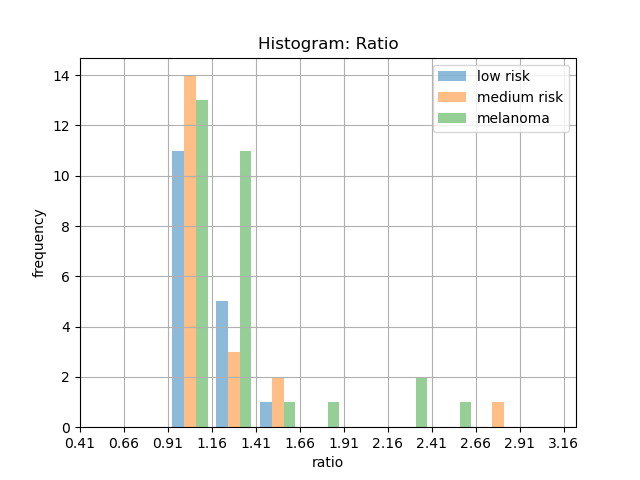
\includegraphics[scale=0.35]{histograph.png}
		
		\caption{Histogram reporting the recurrence of ratio values for low and medium risk moles and melanoma.}
		\label{histo}
	\end{figure}
	
	
	\section{Conclusions}
	As we can see from the results we have obtained, analyzing only the border of a mole isn’t sufficient to make a ‘correct classification’ like: ‘it’s melanoma’ or not. In fact, as said at the beginning, the features of a mole we should analyze to understand its evolution are summarized in the acronym ABCDE: A asymmetry; B border; C color; D diameter; E evolution. So, it’s impossible to diagnose a melanoma from a mole only analyzing the perimeter. Despite this, the algorithm we have used works well and gives us a correct result. In fact, as we can see from final results, the ratios from ‘melanoma’ images are, on average, higher than the ones from ‘low risk’ moles, similarly for the ones from ‘medium risk’ moles.
	
	
	
	
\end{document}